\chapter{Lead-lag relationships} \label{chap:lagCorrelation}

Arbitrage traders take advantage of correlations between financial instruments. They try to detect and exploit pricing anomalies.  Such opportunities can arise when the price movements of one asset lags behind those of another. Cross-correlations and lead-lag indicators are important
in trying to find out which asset leads. 

When the assets are known to be correlated traders can make predictions of the eventual price of the lagging instrument and place orders to buy or sell accordingly.  Market makers who post prices in these markets have closely coupled interest since lead-lag relationships will determine the price they are prepared to quote to other traders. For high-frequency trading it is important to determine such effects on very short time scales, since some assets follow the
path of others with a small time lag.  

Lead-lag
effects are not constant throughout the day and may vary from day to day. There is intraday seasonality
associated with specific times such as the announcement of macroeconomic
figures and the US market opening. Strong asymmetric cross-correlation functions
are empirically observed, especially in the Futures and Equities markets. Normally the most
liquid assets with short inter-trade duration, narrow bid-ask spread and small volatility lead smaller stocks. These lead-lag relationships become more and more pronounced
as we zoom in on significant events.

In this chapter we start by looking at established methods for measuring lead-lag effects and illustrate their use, noting that the issue of asynchronicity arises immediately for price determination, as in Chapter 5.  We then focus on lead-lag analysis in low latency trading networks where trigger and response events are discrete and recorded to nanosecond precision. We demonstrate how a detailed picture of lagged response can be built up for communication across competing high-speed networks linking multiple exchanges. We then develop and implement an algorithm to deal with confounding effects arising from closely spaced trigger events.

\section{Choice of observables}
There are many ways of defining `price' and `observation time' when working with financial time series derived from exchange sources. Lead-lag relationships are highly dependent on the observational framework chosen.  As previously explained in Section \ref{sec:observables}, price can be a simple mid-price or a weighted mid-price, weighting inversely by the volume of asset available at the quoted bid and offer prices.  More elaborate combinations of prices and volumes at various depths in the order book are also utilised. 

As we will see below, the advantage of working with quoted prices and volumes is that they are available continuously in time. The disadvantage in practice is that the associated datasets are large.  Changes in quoted prices and volumes may be fleeting, existing for fractions of a second before the quoted price and volume is modified or cancelled. Such behaviour is reminiscent of the promotional FX prices on Reuters screens as witnessed by \citet{zhou1996high} in the days of telephone trading. 

Alternatively the prices of completed trades can be used. These will move between the bid and offer prices depending on whether the trader is buying or selling -- giving rise to the well known bid/ask bounce effect \citep{roll1984simple}.  To deal with these fluctuations the quoted mid-price at the time of the trade can be used. Another possibility is to use prices generated by the `uncertainty zone' methods of \citet{robert2012volatility}. 

There are also many options in defining timestamps that will serve as the observational clock.  The times when trades occur is an obvious candidate. The times when the mid-price moves is another. High-frequency traders will also look at the BBOT (best bid/offer and trade) timestamps, the times when the quoted volumes at the best bid and offer prices change, either because volume has been added or cancelled or a trade has occurred.  


\section{Measuring lead-lag for prices}
As in Chapter 5, we suppose that there are two assets A and B with prices $X$ and $Y$ that are recorded at discrete times
$\mathcal{T} = (t_0,\dots,t_{m})$ and
$\mathcal{U} = (u_0,\dots,u_{n})$. For lead-lag analysis, we would like to know how the association between the returns of $X$ and $Y$ changes when the timestamps of $Y$ are shifted relative to the timestamps of $X$. In other words how the association between the returns of $X(t)$ and  $Y(t+h)$ changes with lag $h$.  

Covolatility can be used as a measure of association. In Chapter 5 we discussed how to estimate covolatility in the case $h=0$.  In principle these methods can be adapted to estimate the covolatility between the returns of $X(t)$ and $Y(t+h)$ for any value of $h$.

\subsection{Synchronous data}
The simplest case is when $\mathcal{T} = \mathcal{U}$ and the observation times are equally spaced with spacing $\Delta$. This arrangement is possible  when using quote data and only observing the quoted prices at a sequence of times $i\Delta, i = 0,1,\dots$.  In this case the lagged cross-covariance between the return sequences with lags $h = k\Delta$ provides a basic measure of association so that the effect of changing $h$ can be investigated

%
\subsection{Asynchronous data}
More generally covolatility can be estimated using any of the methods in Chapter 5. In particular, shifting the observation times of $Y$ by $h$, the lagged ZHY estimator becomes:
$$ \text{\rm ZHY}(h) = \sum_{ij} R_i S_j(h) \mathbb{I}(\tau_{ij}(h)>0),\quad h \in \mathbb{R},$$
where 
$$S_j(h) = Y(u_j +h)- Y(u_{j-1} + h)$$ and 
$$
 \tau_{ij}(h) = |J_i^X \cap (u_{j-1} +h, u_{j} + h)|,
$$
is the length of the intersection between $J_i^X$ and $(u_{j-1} +h, u_{j} + h)$, i.e.\  the $j$th return interval of $Y$ shifted by the amount $h$. 
See Section \ref{sec:ZHYdefns} for definitions of $J_i^X$, etc.  As in previous Chapters, a physical or TTS clock can be used.

In summary, the ZHY estimator is computed using lagged observations where the times of $Y$ are shifted by $h$. By plotting ZHY$(h)$ against $h$, the values of $h$ that maximise ZHY$(h)$ can be determined.  This approach was suggested by \citet{hoffmann2013estimation} and further studied by \citet{huth2014high} and \citet{alsayed2014ultra}.  Huth and Abergel suggest assessing the strength of lead-lag by comparing the areas under ZHY$(h)$ on either side of zero.  They show that this measure is related to the notion of Granger causality \citep{granger1969investigating}. 

Other measures of covolatility can be adapted in a similar manner, see for example \citet{de1997high} and references therein. \citet{alsayed2014ultra} compare the performance of the ZHY$(h)$ lead-lag estimator with an estimator based on the previous tick (PT) covariance estimator. They show that the PT covariance produces biased estimators of $h$ when one of the assets is observed more frequently than the other. By contrast the ZHY based estimator they advocate is shown to be unbiased. 

In their theoretical analysis, \citet{huth2014high}, assume that log-prices move as correlated Brownian motion and that observation times are drawn from independent Poisson processes. In the same paper they construct the ZHY($h$) plot for French equity and Index Futures data and show that 
the next midquote movement of a stock can be predicted from the past evolution of the Index Futures with high probability.

\subsection{Comparison with extended ZHY}
We follow \citet{huth2014high} and simulate log-prices $(X(t),Y(t+h))$ as correlated Brownian motions with zero means and constant parameters $\sigma_1 = \sigma_2 = 1$ and $\sigma_{12} = 0.9$. The processes are assumed to run on physical time measured in seconds and for the simulation study, $h$ is chosen to be $0.2$ seconds.  Again following \citet{huth2014high} observation times for $X$ and $Y$ are taken from independent Poisson process with rate parameters $\lambda_1$ and $\lambda_2$, respectively.  For a similar setup, see Section \ref{sec:noisefree}.  

\begin{figure}[!ht]
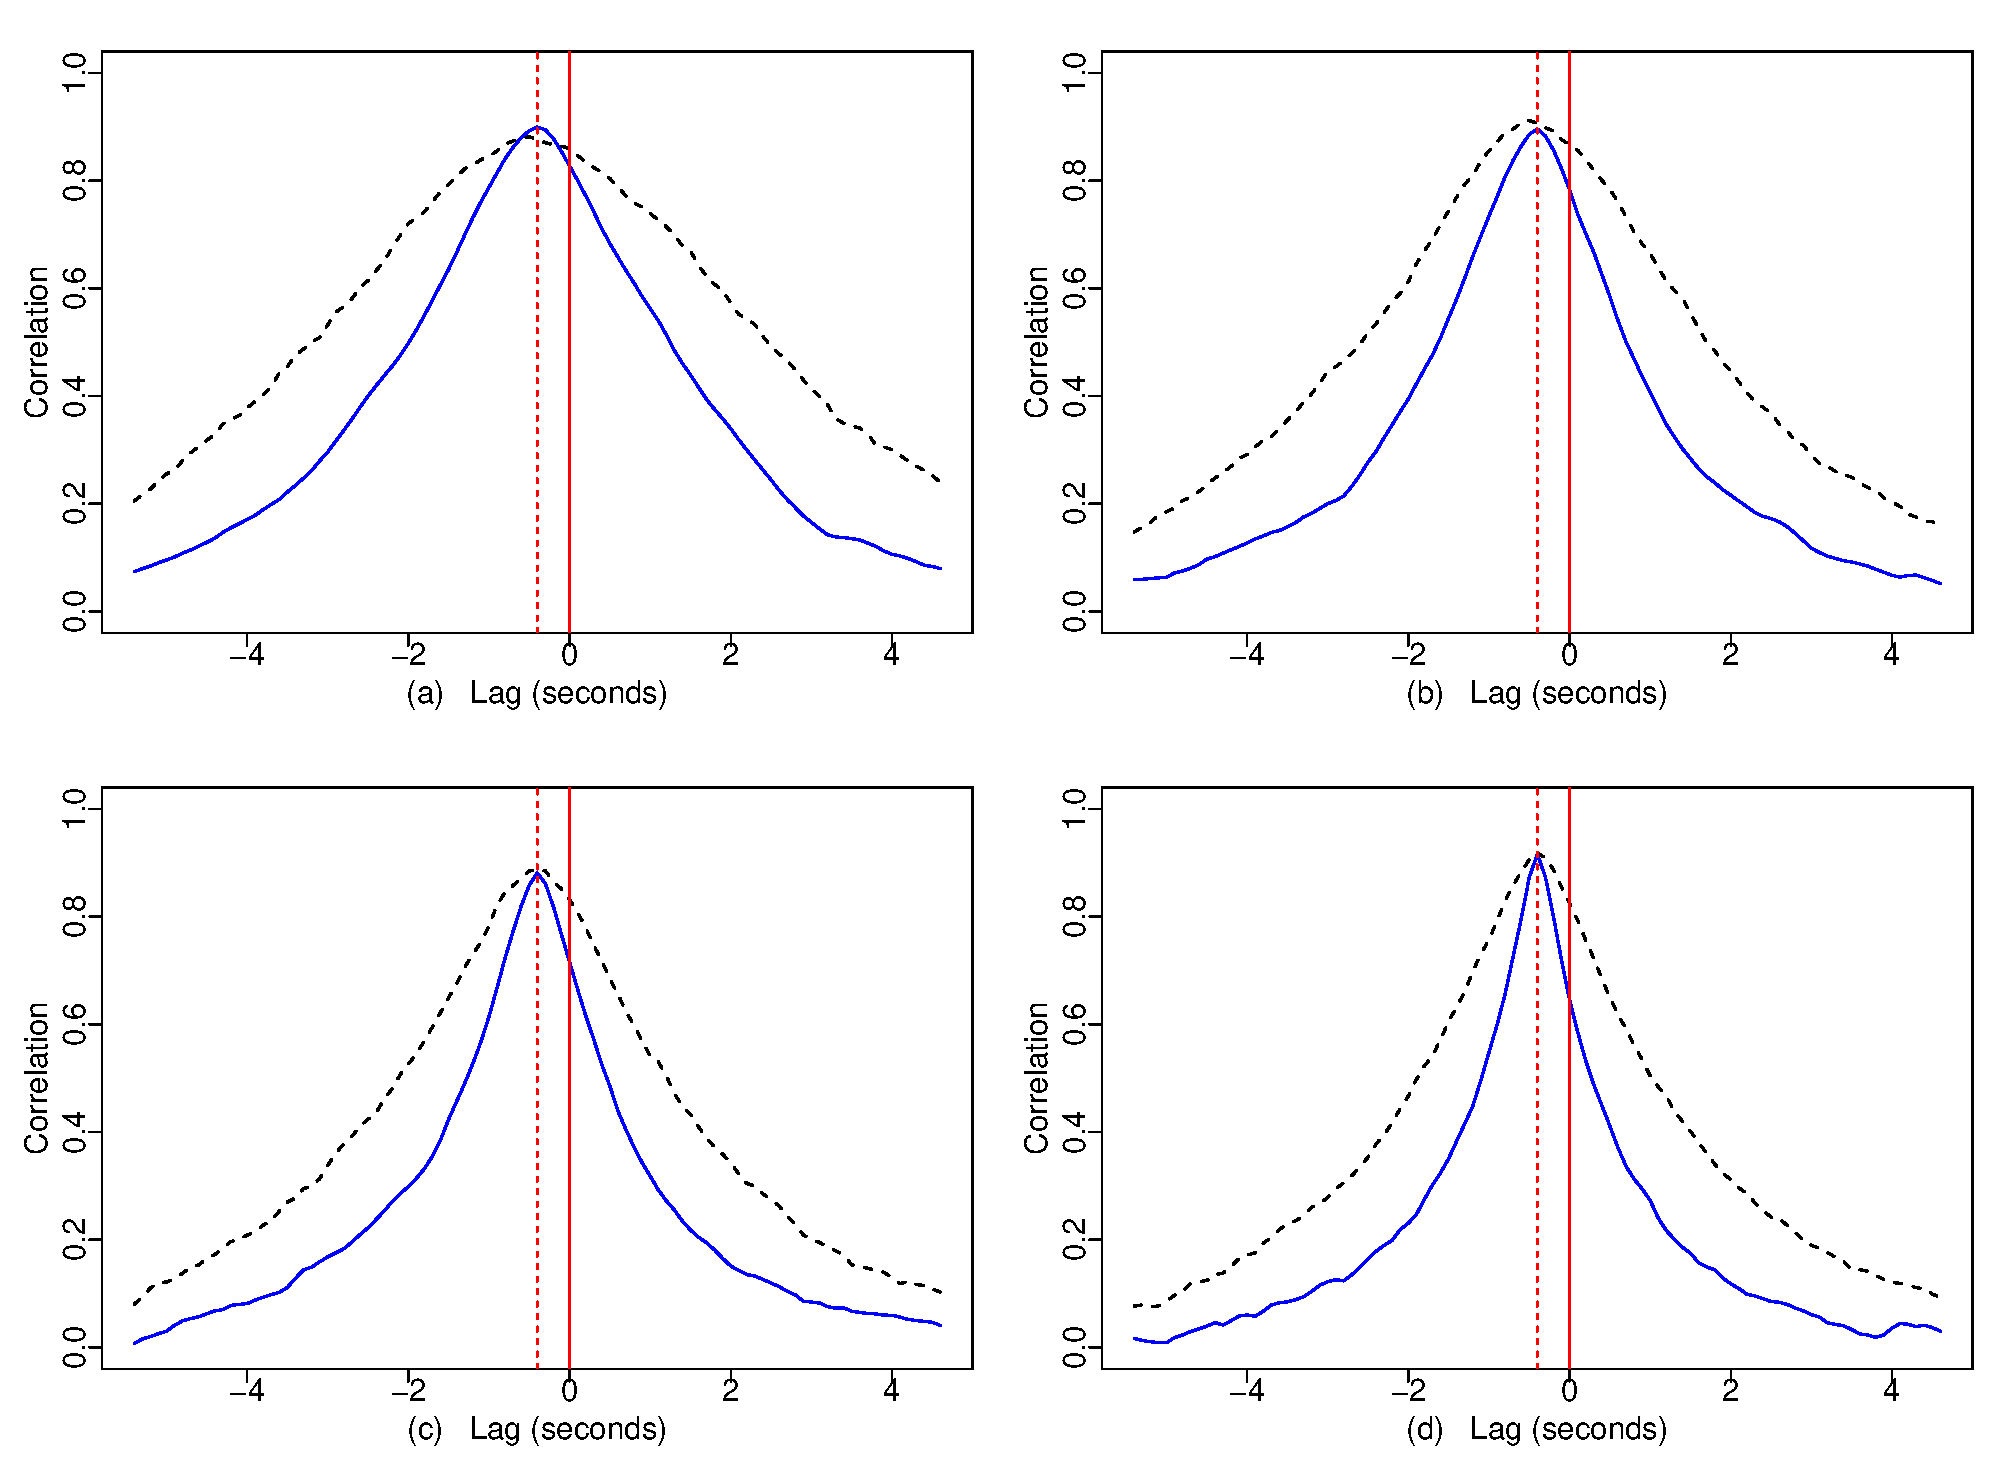
\includegraphics[width=\linewidth]{./Figures/ZHYPoissonBM.pdf}
\caption{Comparison of simulated lead-lag profiles obtained with ZHY$(h)$ and the extended ZHY estimator of Section \ref{sec:specialcase}. The dashed curves are ZHY$(h)$. The ratios $\lambda_1/\lambda_2$ are 1, 2, 5 and 10 in (a), (b), (c) and (d), respectively. The dashed vertical line corresponds to the known lag $-0.2$ secs. \label{fig:ZHYPoisBM}}
\end{figure}

Figure \ref{fig:ZHYPoisBM}, compares the performance of the standard ZHY based estimator used by Huth and Abergel (2014)  with the extended ZHY developed in Section \ref{sec:specialcase}. 

It is clear that our extended ZHY provides a sharper estimate of the known lag under these model assumptions.
\subsection{Application -- Index Futures}
Figure \ref{fig:ZHYhCmeEurex} shows the extended ZHY$(h)$ plot for recent Futures data where asset A is the S\&P 500 E-mini Futures contract traded on CME in Chicago and B is the Euro Stoxx Index Futures contract traded on the Eurex exchange in Frankfurt. The data are mid-prices at the time of trades. If the peak is at a negative value, it indicates that on average Frankfurt price movement is delayed relative to Chicago activity.
\begin{figure}[!ht]
\centering
  \begin{subfigure}[l]{0.49\textwidth}
    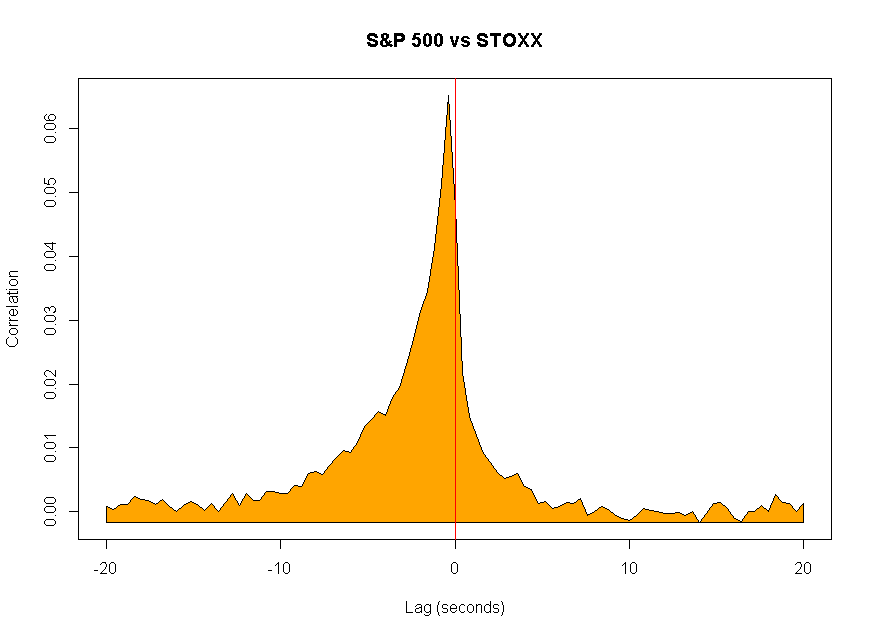
\includegraphics[width=\textwidth]{./Figures/TradesHYRobustMidPrice1013-17sht20000000.png}
    \caption{Week 1}
    \label{fig:ZHYa}
  \end{subfigure} 
  \begin{subfigure}[l]{0.49\textwidth}
    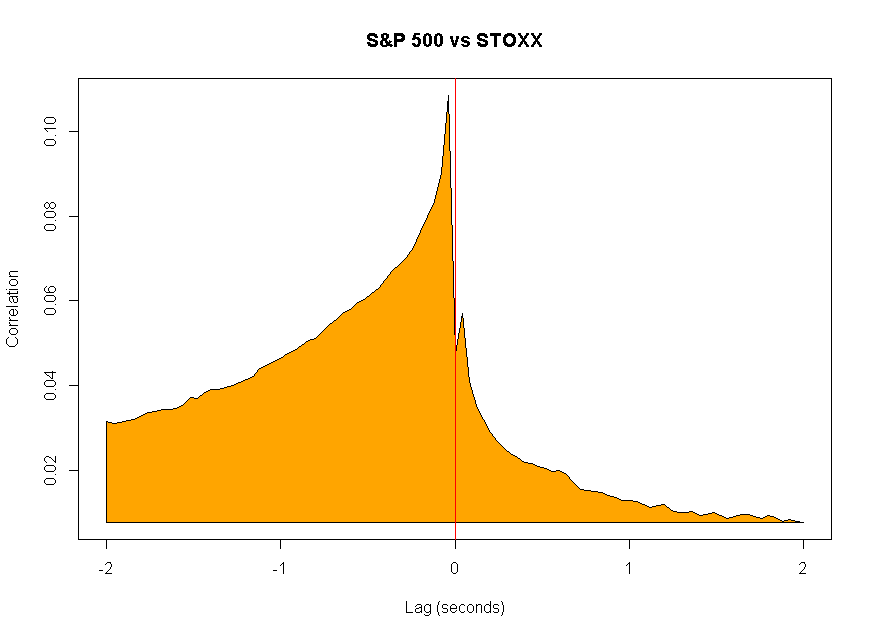
\includegraphics[width=\textwidth]{./Figures/TradesHYRobustMidPrice1013-17sht2000000.png}
    \caption{Week 2}
    \label{fig:ZHYb}
  \end{subfigure}
  
  \begin{subfigure}[l]{0.49\textwidth}
    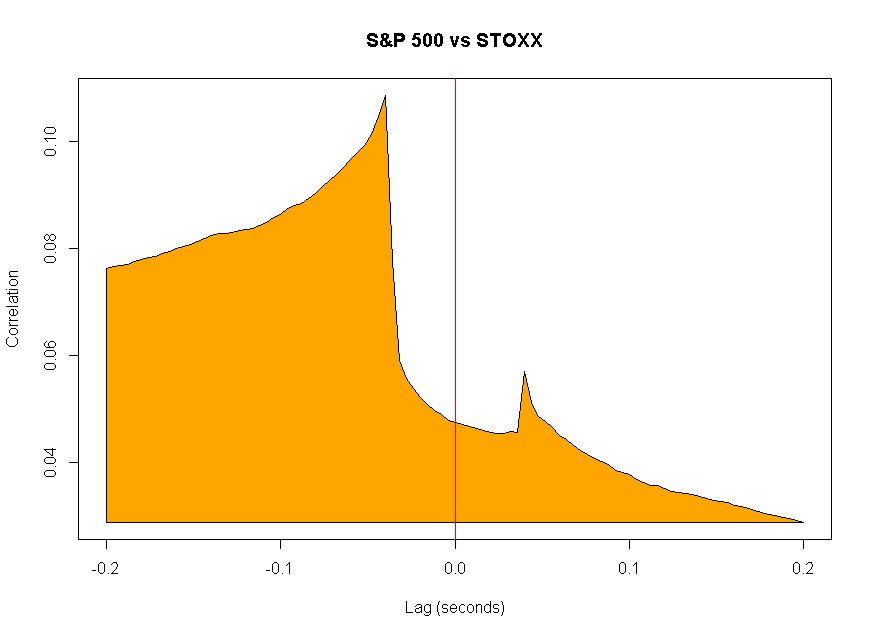
\includegraphics[width=\textwidth]{./Figures/TradesHYRobustMidPrice1013-17sht200000.png}
    \caption{Week 1}
    \label{fig:ZHYc}
  \end{subfigure} 
  \begin{subfigure}[l]{0.49\textwidth}
    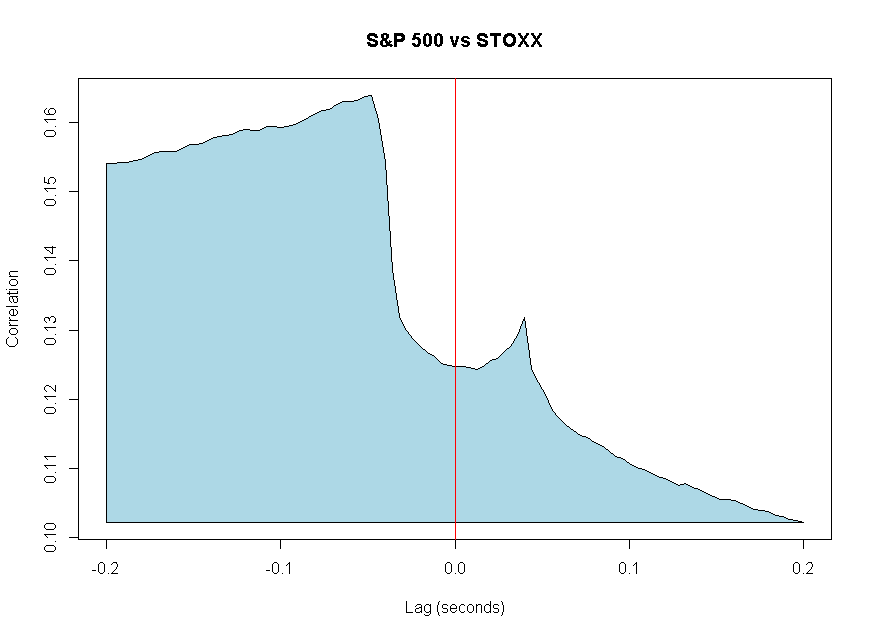
\includegraphics[width=\textwidth]{./Figures/TradesHYRobustMidPrice11215-19sht200000.png}
    \caption{Week 2}
    \label{fig:ZHYd}
  \end{subfigure}
  \caption{Lead-lag plots with the extended ZHY covariance of Section \ref{sec:specialcase} for S\&P 500 Futures in Chicago versus Euro Stoxx Futures in Frankfurt -- two weeks in 2014. Prices are mid-prices at the times of trades. Plots are shown for two time resolutions. \label{fig:ZHYhCmeEurex}}
\end{figure}
\newpage
The broad picture is clear -- namely that the Chicago Futures contract leads the Frankfurt Futures contract. The major peak is around $h = -50$ milliseconds, indicating that Frankfurt responses to Chicago activity are delayed by this amount on average.  There is also a minor peak at $h = 50$ milliseconds, indicating that less commonly  
what happens in Frankfurt will have some impact on what happens in Chicago.

It is also clear that Figure \ref{fig:ZHYhCmeEurex} does not resemble the plots in Figure \ref{fig:ZHYPoisBM}, made under Poisson tick time, Brownian price assumptions. 
\begin{figure}[!ht]
\centering
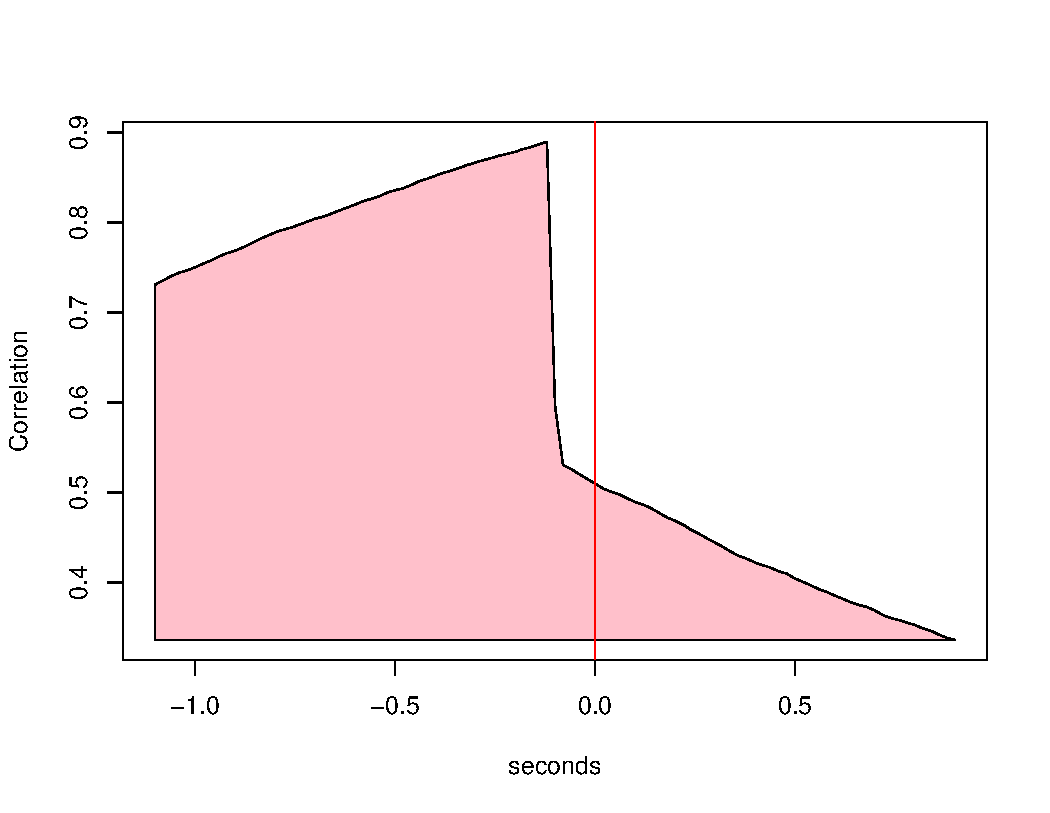
\includegraphics[width=0.6\linewidth]{./Figures/chap5AsymResponse.pdf}
\caption{Simulated asymmetric lead-lag plot where lag is introduced in both tick and calendar time. See text for details of the simulation. \label{fig:chap5AsymResponse}}
\end{figure}
A possible explanation lies in the discrete nature of time at this atomic level of analysis. Brief bursts of activity are followed by relatively long periods with no trades. Lead-lag effects may be more sensibly described in tick time as illustrated in Figure \ref{fig:chap5AsymResponse} and described below.

Suppose that $\{t_i\}$ is a sequence of tick times and that $\{Z_i\}$ and $\{Y_i\}$ are associated random price sequences with $(Z_i - Z_{i-1},Y_{i}-Y_{i-1})$ iid pairs of correlated bivariate normal variables. Now let $X_i = Z_{i+1}$, so that $X$ leads $Y$ by one tick in tick time (TTS). The simulation in Figure \ref{fig:chap5AsymResponse} shows what happens when the ZHY$(h)$ plot is calculated.  Asymmetric behaviour similar to Figure \ref{fig:ZHYhCmeEurex} is reproduced. 

Other explanations in terms of auto-correlation effects are possible. See for the example the references in \citet{griffin2011covariance} relating to controlling lead-lag bias in covariance estimation. Why does it have asymmetric behaviour? To be honest we don't really
know. This will be a very interesting area for further research.

\section{High-frequency lead-lag}\label{sec:HFleadlag}

Competitive performance is a major concern for high-frequency traders who invest substantial amounts of money in leasing or  building their own fast connections between exchanges.  The introduction of fibre-optic and microwave connections between exchanges marked major steps in improving connection latency. Nowadays, high-speed connections can transmit data between Chicago and Frankfurt in under 40 milliseconds. The bulk of the transmission time is taken up by the transatlantic portion of the route. Around a dozen transatlantic cables are  available, running between New York and the cable landing point near Bude in Cornwall, UK. Faster microwave networks link Chicago with New York and link Bude to London, down to Dover, across the Channel and then on to Frankfurt 
\citep{amsterdamtrader1,amsterdamtrader2}.

The broad picture provided by our ZHY$(h)$ plot is not able to expose the detailed micro-structure of high-speed lagged responses. High-frequency traders want to know how much slower or faster their connections are than others, i.e.\ what is the latency profile of competitors between specific exchanges.  In the next section we demonstrate how to reveal this profile, discuss possible weaknesses and propose and implement an improved method.

\subsection{Event-based latency profiles}
The objective is to investigate the different network and infrastructure speeds used by high-frequency trading firms when communicating between the major financial  exchanges. 
A very simple way to do this is to wait for a large trigger trade in Chicago for example, then see how soon people trade in the same direction in other exchanges such as  New York, London and Frankfurt after this
event. 

If a significant event occurs in Chicago, e.g.\ some large trade
at a particular time, traders in Frankfurt will receive the signal
at different times, depending on how fast their network connection and trading infrastructure is. We would like to build
a latency profile for their responses. 

\subsection{Exploratory analysis}
Our first proposal exploits the bursty nature of trade data. S\&P 500 Futures trades in Chicago can be viewed as trigger events. The times between trades of Futures contracts on CME have a heavy tailed distribution. 
We can find numerous S\&P 500 Futures trades that are separated from trades of the same contract by significant gaps of time, both before and after. 
Treating these special trades as triggers we can look at potential BBOT (best bid, offer and trade) responses involving the Euro Stoxx contract in Frankfurt for example, i.e.\ trades, addition, cancellation or modification of volume at the best prices. For each such event we look back to the most recent Chicago trigger event and prepare a histogram of the elapsed time between the trigger and the response. 

Figure \ref{fig:SimpleSP500TradeEurex} shows the result of such a calculation. Basic features of the response profile can be identified: the first peak, a peak at around 39 milliseconds corresponding to high-frequency traders with comprehensive microwave connectivity in Europe and the US and the second  peak, a lesser peak at around 45 milliseconds corresponding to slower fibre-optic connection on the mainland routes. There is an intermediate peak for traders who have sub-optimal microwave connections. Responses prior to 35 milliseconds are background noise. 


\begin{figure}[!ht]
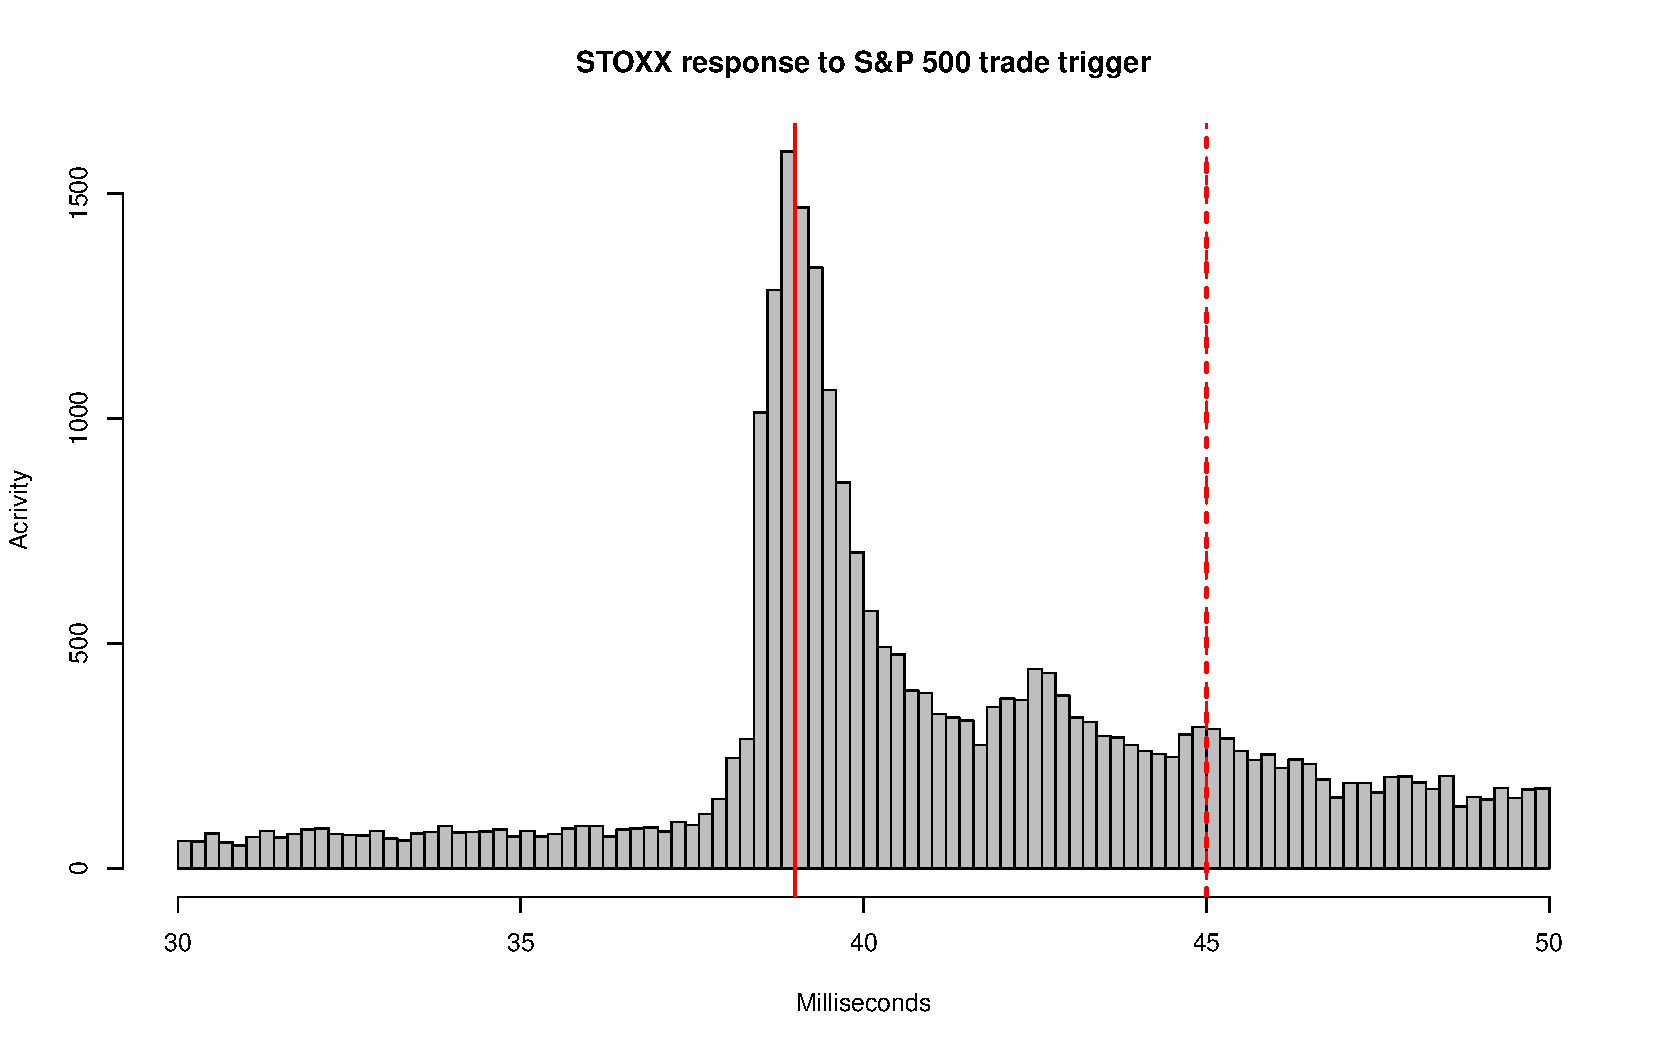
\includegraphics[width=0.9\linewidth]{./Figures/SimpleSP500TradeEurex.pdf}
\caption{Response delay for BBOT activity of Euro Stoxx Futures  with sparse S\&P Futures triggers, for a typical day early in 2014. \label{fig:SimpleSP500TradeEurex}}
\end{figure}
Figure \ref{fig:SimpleSP500TradeEurex} is not a very complicated profile. What are much more interesting are the European
profiles. For example, from Stockholm to Milan, there are several routes one can take: 
go through London or go by Zurich or go by Frankfurt or by Paris. From North Europe to
South Europe, one can get a very complicated latency profile.  Investigation of such profiles is commercially sensitive and requires access to high-precision transaction timestamps at multiple exchanges.

\subsection{A theoretical framework}\label{sec:EMassumptions} 
Although there are many Chicago trades that fit our separation criterion, there may be concern that their impact on the response profile is not representative of all trades. The problem is that unseparated trades may produce responses that overlap with responses from other trades that are close in time.  

The simple histogram plot is not able to separate noise from signal. From Figure \ref{fig:SimpleSP500TradeEurex} we can see, there is a lot of noise before 35
millisecond and also a lot of noise in the tail too. Before 35 millisecond, this is nearly
certainly background noise. The problem is how to eliminate the noise.

To formalise the problem we denote the sequence of trigger times at exchange A by $\mathcal{T} = (t_1,\dots,t_m)$, i.e.\ the trigger times at exchange A are $t_1$ to $t_m$. Each trigger independently produces a cluster of delayed responses at exchange B.   
i.e.\ each trigger independently produces a cluster of delayed
responses from trading company $x$, trading company $y$, trading company $z$, etc. Different trading companies will respond at different times, depending on what kind of network speed they
have. The number of responses is not fixed. It will be variable depending for example
on the size of the trigger trade, or the state of the trading company's inventory or position.  Of course a trading company may decide not to
respond at all, so
the number of responses that each trigger produces will change depending on circumstances.

To allow for this variability, we model the number of responses for each trigger as a Poisson variable with mean $\mu$. 
We also assume that individual response delays for each trigger are drawn independently from a distribution $F$, i.e.\ the individual response
delays vary between different trading companies; some respond fast and some respond slow. As a consequence, there is pattern of events generated in exchange B, every time there is an event in exchange A. 

In addition there will be responses at exchange B that are not the direct result of activity on exchange A.   These arise from people trading on exchange B using information that does not come from exchange A. We call this background. For example, activity in Frankfurt will come from internal behaviour of the market in Frankfurt, or information from
New York, London, Paris, Milan or wherever it is. So there will be events
which are not triggered by Chicago. To accommodate this, we suppose that independently there will be untriggered background events at exchange B and that these form a Poisson process with constant intensity $\lambda_0$. This noise is not what we are interested in.  We are interested in the response to the Chicago trigger. Our objective is then to estimate $\mu, F, \lambda_0$.

Although we would like to do everything in continuous time, for now we are
going to switch to discrete time.  To make progress with our formulation we will assume that $\{t_i\}$ and the response times take discrete values on a regular grid with grid points numbered in $\mathbb{N}$. We are just going to round all the times to the nearest $q$ microseconds, so
our clock will just tick every $q$ microseconds. Therefore, we get a distribution
on that discrete time scale with a probability mass function. For high-frequency applications we take the grid width to be around $q=100$ microseconds.  The delay distribution $F$ is assumed to have finite support with probability mass function $\{p_k, k = 1,\dots,d\}$. 

Figure \ref{fig:chap5problem} illustrates what might be observed with events occurring in Chicago and some
events occurring in Frankfurt.
\begin{figure}[!ht]
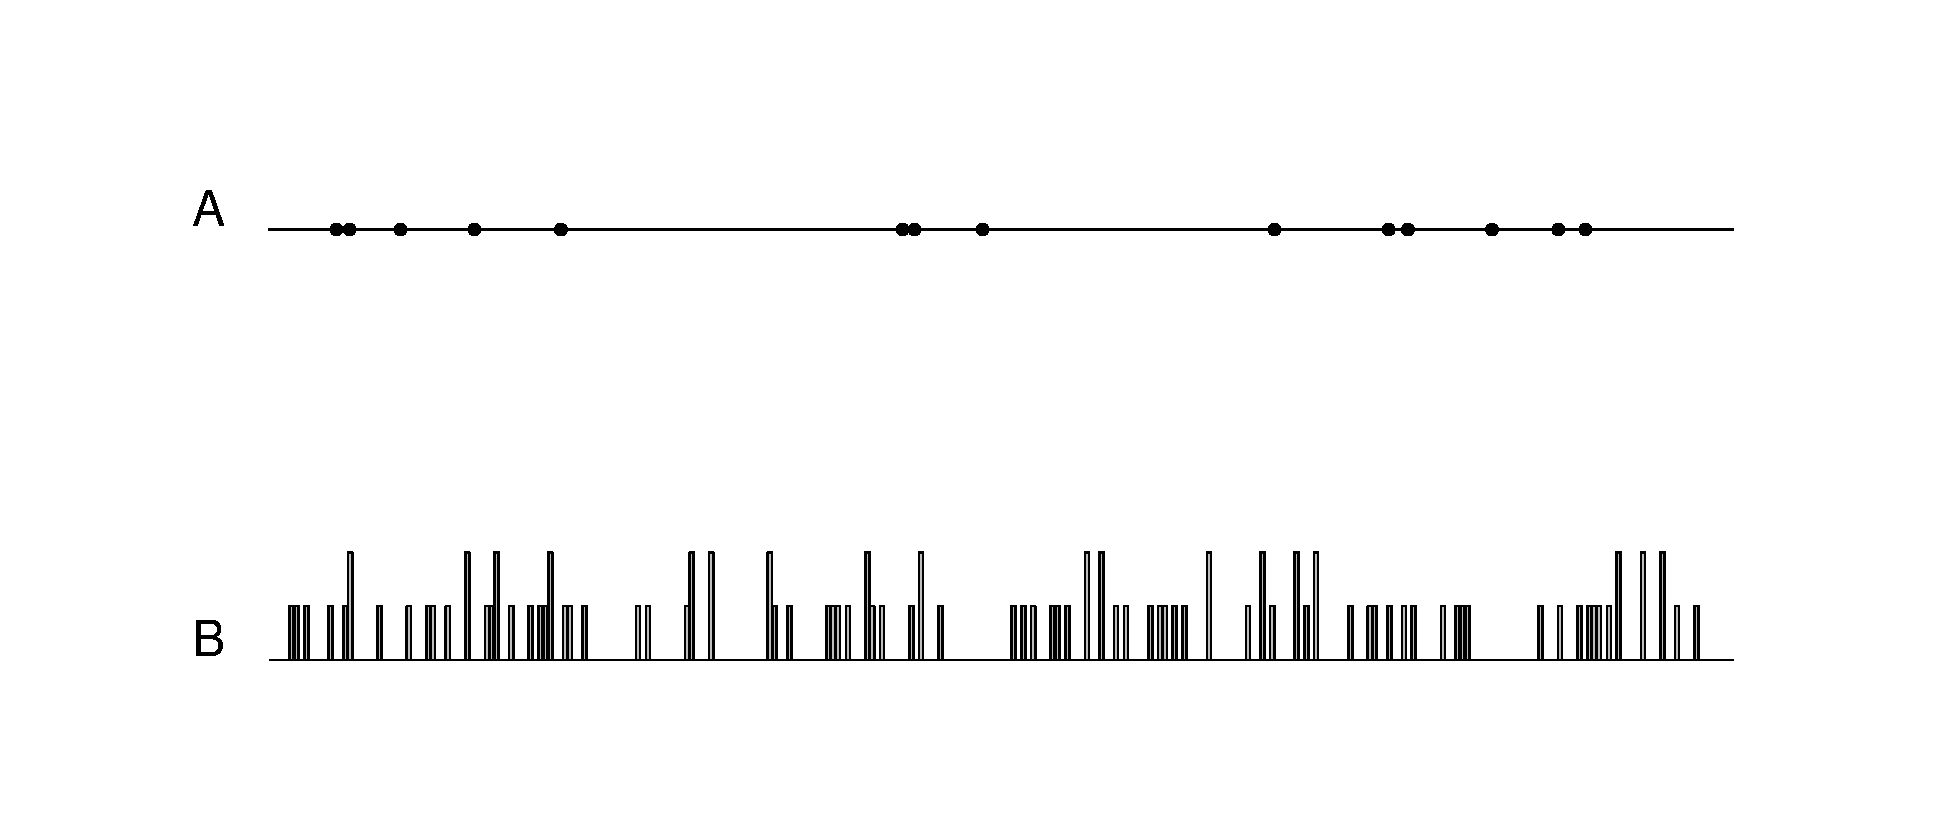
\includegraphics[width=0.9\linewidth]{./Figures/chap5problem.pdf}
\caption{The events at exchange B are either delayed responses to triggers on A or background noise. BBOT responses on B will outnumber trade triggers on A. \label{fig:chap5problem}}
\end{figure} 

The idea is to figure out which of the events in B are generated by which of the events in A. If we just look at it, we will have no idea at
all how B relates to A. Our task is to untangle what we see in B and split it into some noise plus some signal.

The input data set is then $\{t_i\}$, the trade times at exchange A, and for each $j$, the number of events $W_j$ at the $j$th grid point on exchange B as illustrated in Figure \ref{fig:chap5problem}.  

Futures exchanges have substantial activity for around 14 hours a day so $N$ the number of 100 microsecond grid points is around half a billion. Our main interest is in estimating the response profile, $\{p_k, k = 1,\dots,d\}$ where $d$ is a few hundred.

We know the structure of $W_j$.  It is the sum of background noise (with parameter $\lambda_0$) plus contributions from events that occurred in exchange A, taking into account the latencies of different participants. These contributions have a Poisson distribution depending on parameters $p$ and $\mu$.  The likelihood of the parameter set $(p, \mu, \lambda_0)$ becomes a simple product of Poisson likelihoods.  

Since $W_j$ is the sum of independent Poisson variables with contributions from each of the triggers and the background, it has a Poisson distribution with mean $\mu_j$  where
\begin{equation}
\label{eq:PoissonMean} 
\mu_j = \lambda_0  + \mu \sum_{j-d \leqslant r \leqslant j} p(j - r + 1)\mathbb{I}_r,
\end{equation}
where $\mathbb{I}_r = 1$ when $r \in \mathcal{T}$ and zero otherwise.  Since the contributions to each of the elements of $\{W_j\}$ are independent, the likelihood of $p,\mu, \lambda_0$ given $\{W_j = w_j\}$ is
\begin{equation}\label{eq:EMMLE}
L(p,\mu,\lambda_0) = \prod_{j=1}^N \frac{\text{\rm e}^{-\mu_j} \mu_j^{w_j}}{w_j!}.
\end{equation} 
Direct optimisation is unrealistic but with the aid of a short cut we will show that the EM algorithm provides a practical solution.

\subsection{Optimisation}
For convenience let $\lambda_k = \mu p_k, k =1,\dots,d$.  Now note if we have available $Z^{(s)}_k$, the number of responses triggered at time $s$ that arrive at time $s+k-1$ for $s \in \mathcal{T}$, then we can estimate $\lambda_k$ directly as
\begin{equation}\label{eq:lambdak} \hat{\lambda}_k = \frac{1}{m} \sum_{s \in \mathcal{T}} Z_k^{(s)},\end{equation}
since $\{Z^{(s)}_k, s \in \mathcal{T}\}$ are independent Poisson variables each with mean $\lambda_k$. Similarly, the background rate $\lambda_0$ can be estimated by
$$\hat{\lambda}_0 = \frac{\sum_{j=1}^N \left(W_j - \sum_{s \in \mathcal{T}} Z^{(s)}_{j-s+1}\right)}{N},$$
since when the triggered responses have been removed only the background events remain and these are independently Poisson with mean $\lambda_0$.

To apply the EM algorithm to maximise \ref{eq:EMMLE} we proceed as usual to find the expected value of the log likelihood which in this case is the sum of log likelihoods for the independent Poisson components. Since the distributions are Poisson this reduces to finding terms like $\EE(Z^{(s)}_k | W)$, with     
\begin{equation}\label{eq:sumW}
W_j = \sum_{s \in\mathcal{T}} Z^{(s)}_{j-s+1} + B_j,\quad j = 1,\dots,N,
\end{equation}
where $B_j$ is the unobserved background count. We see that $Z^{(s)}_k$ appears in $W_j$ only when $j = s+k-1$.  

From \eqref{eq:sumW} since $W_j$ is the sum if independent Poisson components $\{Z^{(s)}_{j-s+1}, s \in \mathcal{T}\}$ and $B_j$, with means $\{\lambda_{j-s+1}$, $s \in \mathcal{T}\}$ and $\lambda_0$, respectively. It follows that 
$$ \EE(Z^{(s)}_{j-s+1} | W) = \EE(Z^{(s)}_{j-s+1} | W_j) = \frac{\lambda_{j-s+1}}{\EE(W_j)} W_j, \quad s \in \mathcal{T},$$
so that 
\begin{equation}\label{eq:ExpZ} \EE(Z^{(s)}_k | W) = \frac{\lambda_{k}}{\EE(W_{k+s-1})} W_{k+s-1}, \quad s \in \mathcal{T}.\end{equation}
and similarly
\begin{equation}\label{eq:ExpB} \EE(B_j|W) = \frac{\lambda_0}{\EE(W_j)} W_j,\end{equation}
where 
\begin{equation}\label{eq:ExpW}\EE(W_j) = \sum_{r \in\mathcal{T}} \lambda_{j-r+1} + \lambda_0,\end{equation}
from \ref{eq:sumW}.

\subsection{EM steps}
The EM iteration starts with initial estimates of $\lambda_k,k=0,\dots,d$, denoted by $\{\hat{\lambda}^{(0)}_k\}$. Starting at step $h=0$, the iteration is as follows: 

\begin{itemize}
\item[(1)] Calculate $\EE(Z^{(s)}_k | W)$ using \eqref{eq:ExpZ}, \eqref{eq:ExpB} and \eqref{eq:ExpW} using $\{\hat{\lambda}^{(h)}_k\}$.
\item[(2)] Replace $Z_k^{(s)}$ in \eqref{eq:lambdak} by the calculated values $\EE(Z^{(s)}_k | W)$ to obtain a revised estimate of $\lambda_k$, namely
$$ \hat{\lambda}_k^{(h+1)} = \frac{1}{m}  \sum_{s\in \mathcal{T}} 
\left(\frac{\hat{\lambda}_k^{(h)} W_{k+s-1}}{\sum_{r \in\mathcal{T}} \hat{\lambda}_{k+s-r}^{(h)} + \hat{\lambda}_0^{(h)}}\right),\quad k=1,\dots,d,$$
and 
$$ \hat{\lambda}_0^{(h+1)} = \frac{1}{N}\sum_{j=1}^N \left( \frac{\hat{\lambda}_0^{(h)} W_j  }{\sum_{s \in \mathcal{T}} \hat{\lambda}_{j-s+1}^{(h)} + \hat{\lambda}_0^{(h)}}\right).$$
\item[(3)] Iterate to convergence.
\end{itemize}

The calculation of $\EE(W_j)$ at each step is a key component of the algorithm. The first term in \eqref{eq:ExpW} can be written as 
$$\phi(j) = \sum_{r \in\mathcal{T}} \lambda_{j-r+1} = \sum_{i=1}^N \lambda_{j-i+1} \mathbb{I}_i = \sum_{k=1}^{d \wedge j} \lambda_k \mathbb{I}_{j-k+1},$$
where $\mathbb{I}$ is the indicator defined in \eqref{eq:PoissonMean}.  This means that $\phi$ is a moving average of $\mathbb{I}$, that can be calculated rapidly by the {\sf filter} function in {\sf R}. 

Although the calculation time is linear in $N$ given the size of $N$ this still represents a substantial computing effort. 

However the bursty nature of high-frequency data allows time-savings to be made. This is because any response period longer than $d$ without a trigger event can only contain background noise, assuming $d$ is sufficiently large to cover the range of possible delay times.  Periods longer than $d$ can be truncated without affecting the calculation and the periods that are removed provide a separate estimate of the background rate.    
The pre-processing step is as follows. 
\begin{itemize}
\item[(a)] First fix the grid points. For example set the spacing at $100$ microseconds.     
\item[(b)] Fix the range of response times of interest, say $30000$ to $50000$ microseconds, so that $d = 200$.
\item[(c)] Remove time periods where there is no trigger for $L$ grid points, say $L=1000$, i.e.\  $0.1$  seconds.
\end{itemize}
For a typical daily trading period, 07:00 to 21:00, with the figures as itemized above, the initial size of $N$ is approximately $500$ million. On a reasonably active day there may be $100,000$ trigger events, i.e.\  $100,000$ trades of the S\&P Futures contract in Chicago. Choosing a day at random we found that $35,000$ trades were followed by a gap of at least $0.1$ seconds. The total length of these gaps is $13.8$ hours, i.e.\ most of the day's trading is compressed into 12 minutes! Since there are $7.2$ million grid points in 12 minutes, we have reduced the size of $N$ by a factor of $70$. Further reduction can be achieved by reducing $L$. As a result the modified EM algorithm becomes feasible and runs in a few seconds in {\sf R}.

To illustrate we apply the EM algorithm to the data of Figure \ref{fig:SimpleSP500TradeEurex}. The grid width is taken to be 100 microseconds with $d = 200$. Convergence is extremely rapid, with the basic shape of the profile visible after two iterations. 

There is a general view in the statistical community that the EM algorithm is slow to converge.  This is not the case here. It seems that our model specification is particularly well adapted to the application of the EM algorithm.   

Figures \ref{fig:EMSTOXXSPIter2} and \ref{fig:EMSTOXXSP} show the result of the EM algorithm after 2 and then 20 iterations. Note that the algorithm progressively eliminates unwanted noise as was the original intention.
\begin{figure}[!ht]
\centering
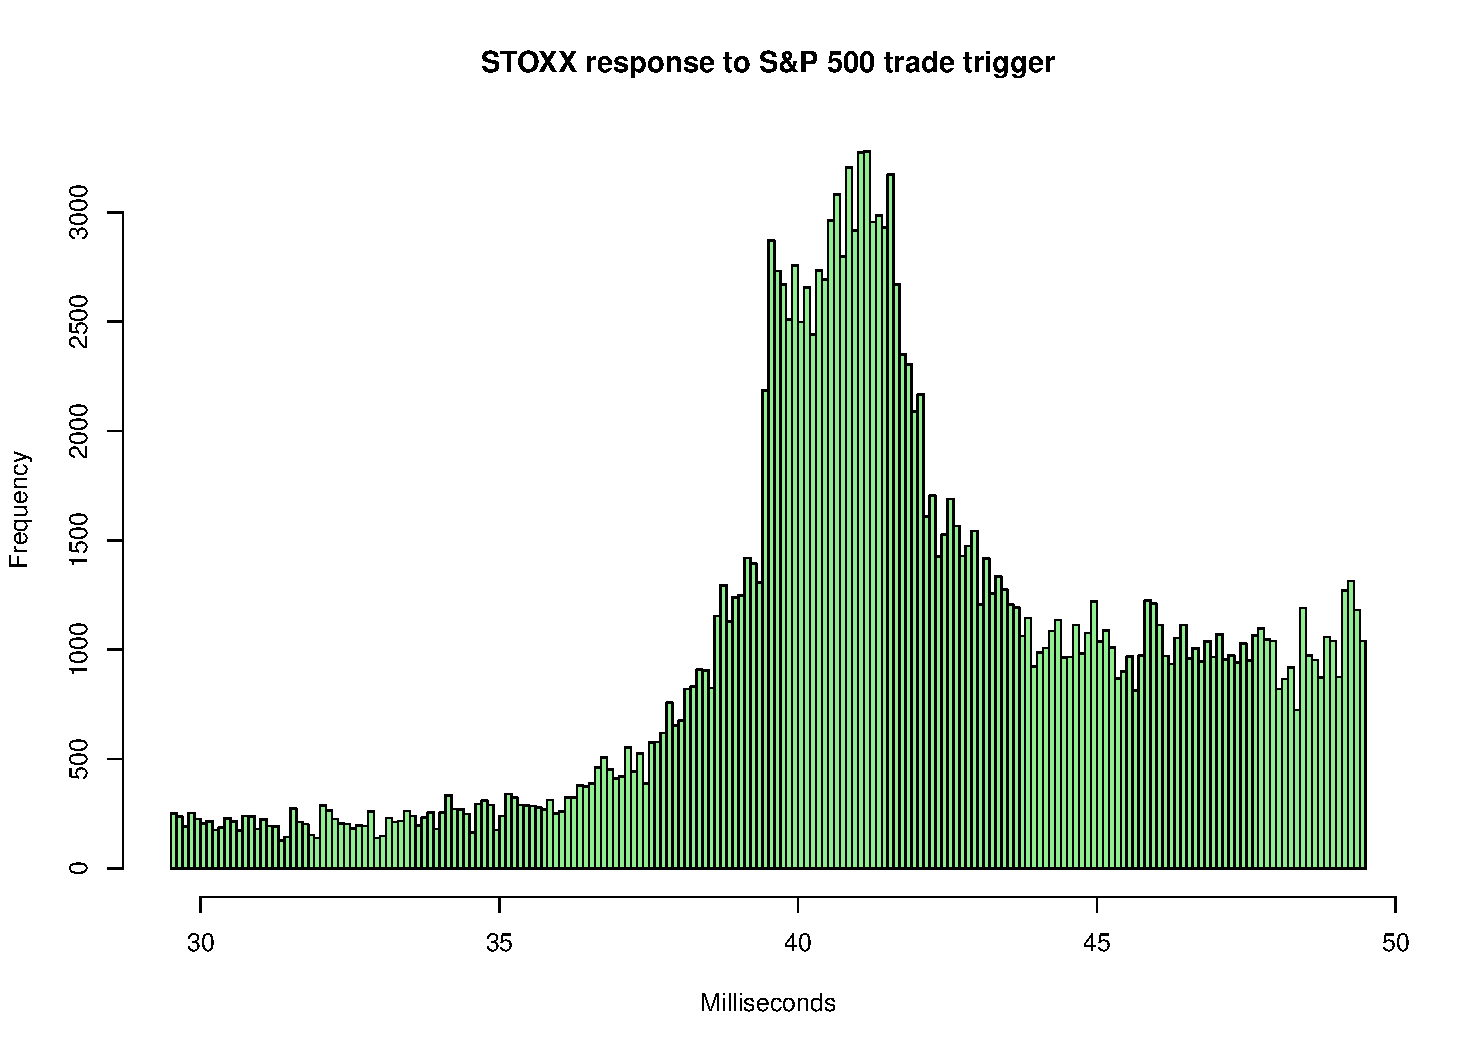
\includegraphics[width=0.8\linewidth]{./Figures/EMSTOXXSPIter2.pdf}. 
\caption{Maximum likelihood reconstruction of the profile of Euro Stoxx Futures responses to trades of S\&P Futures, after 2 iterations of the EM algorithm.  \label{fig:EMSTOXXSPIter2}}
\end{figure}  
\begin{figure}[!ht]
\centering
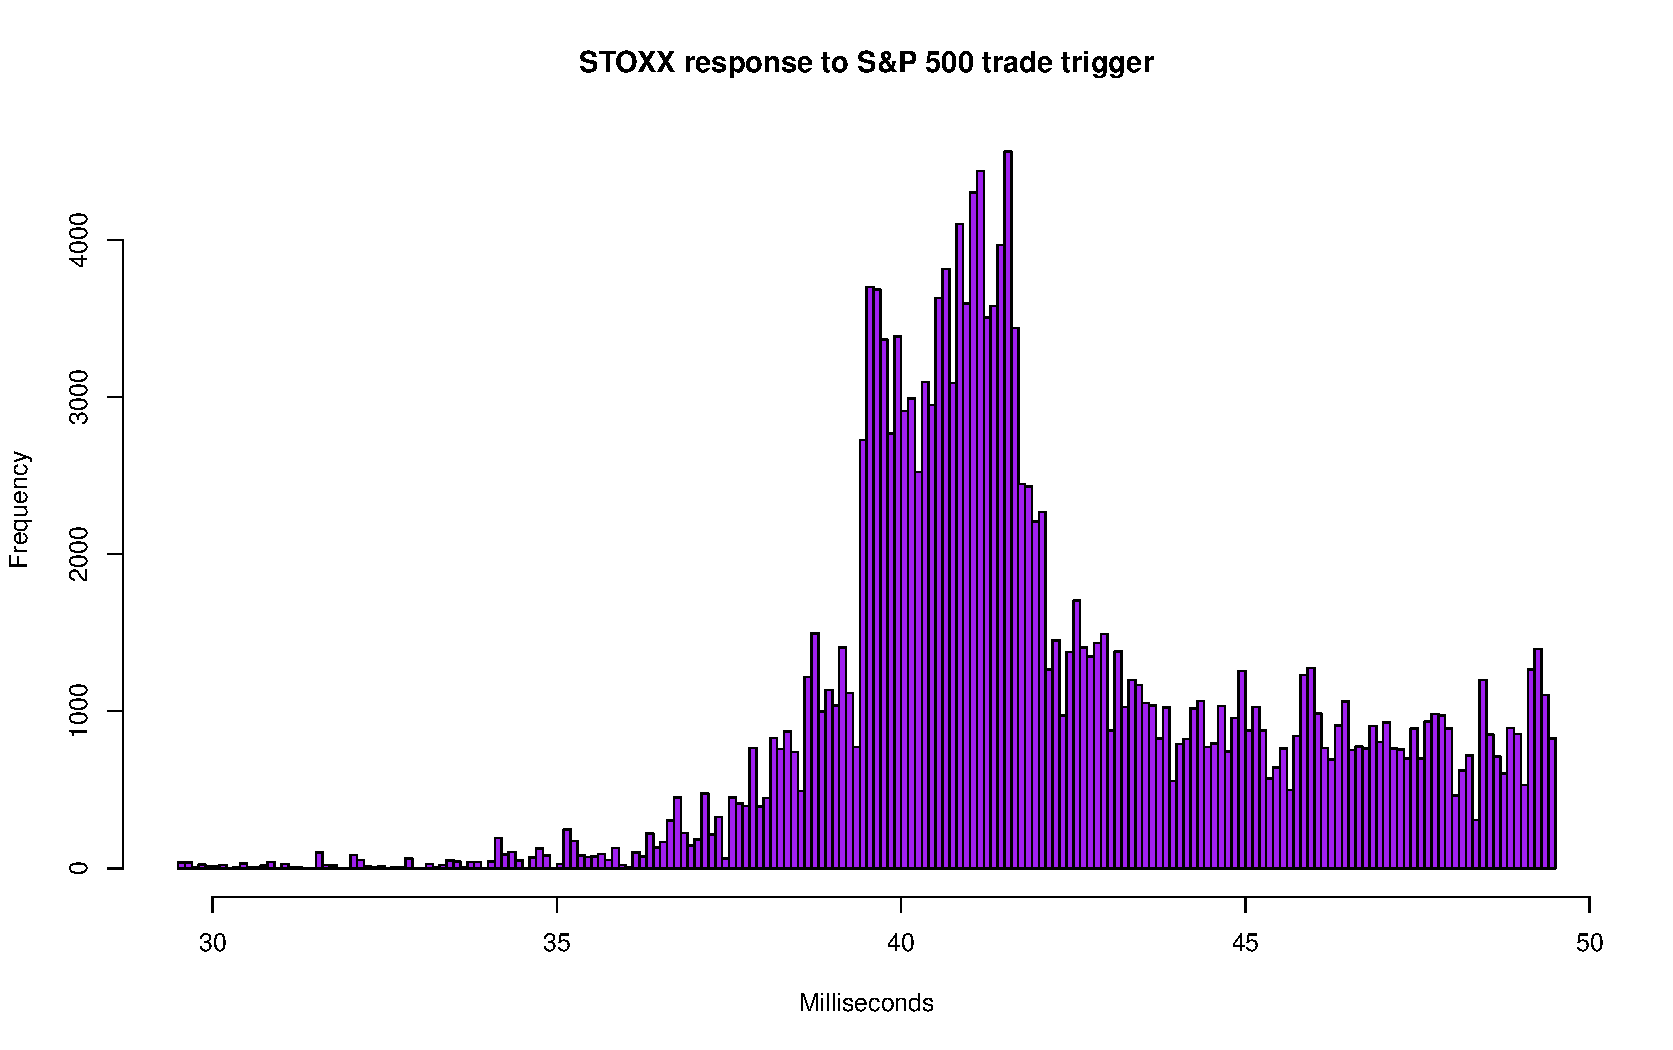
\includegraphics[width=0.8\linewidth]{./Figures/EMSTOXXSP.pdf}. 
\caption{Maximum likelihood reconstruction of the profile of Euro Stoxx Futures responses to trades of S\&P Futures, after 20 iterations of the EM algorithm.  \label{fig:EMSTOXXSP}}
\end{figure}


        
   







  


